\documentclass[tikz]{standalone}
\usetikzlibrary{backgrounds}
\begin{document}
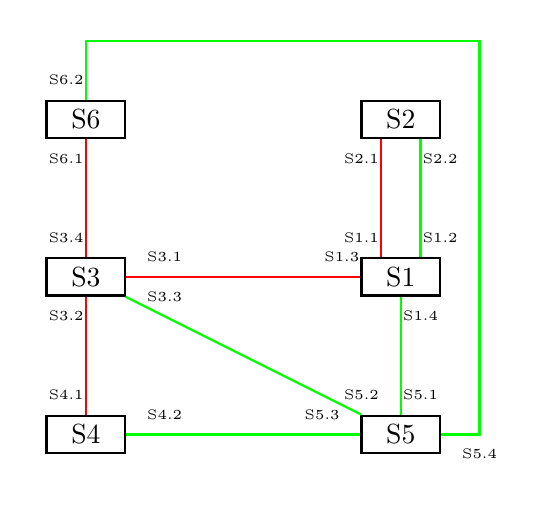
\begin{tikzpicture}[background rectangle/.style={fill=white!}, show background rectangle, -latex ,auto,
semithick ,
state/.style ={thick, rectangle,draw,minimum width =1 cm}],

\node[state] (S6) at (0,0) {S6};
\node[state] (S2) at (4,0) {S2};
\node[state] (S3) at (0,-2) {S3};
\node[state] (S1) at (4,-2) {S1};
\node[state] (S4) at (0,-4) {S4};
\node[state] (S5) at (4,-4) {S5};

\draw[thick,-, color=green] (4.25,-1.75) -- (4.25,-0.25);
\draw[thick,-, color=red] (3.75,-1.75) -- (3.75,-0.25);
\draw[thick,-, color=red] (S1) -- (S3);
\draw[thick,-, color=green] (S1) -- (S5);
\draw[thick,-, color=red] (S3) -- (S4);
\draw[thick,-, color=green] (S3) -- (S5);
\draw[thick,-, color=red] (S3) -- (S6);
\draw[thick,-, color=green] (S4) -- (S5);
\draw[thick,-, color=green] (S5) -- (5,-4) -- (5,1) -- (0,1) -- (S6);

\node (S1.2) at (4.5,-1.5) {\tiny S1.2};
\node (S1.1) at (3.5,-1.5) {\tiny S1.1};
\node (S2.2) at (4.5,-0.5) {\tiny S2.2};
\node (S2.1) at (3.5,-0.5) {\tiny S2.1};
\node (S1.3) at (3.25,-1.75) {\tiny S1.3};
\node (S1.4) at (4.25,-2.5) {\tiny S1.4};
\node (S3.1) at (1,-1.75) {\tiny S3.1};
\node (S3.2) at (-0.25,-2.5) {\tiny S3.2};
\node (S3.3) at (1,-2.25) {\tiny S3.3};
\node (S3.4) at (-0.25,-1.5) {\tiny S3.4};
\node (S4.1) at (-0.25,-3.5) {\tiny S4.1};
\node (S4.2) at (1,-3.75) {\tiny S4.2};
\node (S5.1) at (4.25,-3.5) {\tiny S5.1};
\node (S5.2) at (3.5,-3.5) {\tiny S5.2};
\node (S5.3) at (3,-3.75) {\tiny S5.3};
\node (S5.4) at (5,-4.25) {\tiny S5.4};
\node (S6.1) at (-0.25,-0.5) {\tiny S6.1};
\node (S6.2) at (-0.25,0.5) {\tiny S6.2};


\end{tikzpicture}
\end{document}